\section{Experimental Setup}
\label{sec:expt-setup}


 % Please add the following required packages to your document preamble:
% \usepackage{booktabs}
\begin{table}
\small
\centering
\begin{tabular}{@{}lccc@{}}
\toprule
\textbf{Dataset} & \textbf{Type} & \textbf{Class} & \textbf{Train, Test} \\ 
\midrule
\AGNews   & Topic            & $4$              & $115\text{K}, 7.6\text{K}$           \\
\ToIHeadlines   & Topic            & $10$             & $52\text{K}, 10\text{K}$             \\
\Humor   & Sentiment      & $2$     & $15\text{K}, 3\text{K}$   \\
\IMDb   & Sentiment      & $2$     & $20\text{K}, 25\text{K}$   \\ 
\bottomrule
\end{tabular}
\caption{Dataset statistics.}
\vspace{-1em}
\label{tab:tasks}
\end{table}


% \begin{table}
% \small
% \centering
% \setlength{\tabcolsep}{3pt}
% \begin{tabular}{
% l
% c
% c
% c
% h
% }
% \toprule
% \textbf{Corpus} & \textbf{Domain} & \textbf{Docs} & \textbf{Item} & \textbf{Tokens} \\ \midrule

% \RealNewsDom    & US/EU News    & $30.1\text{M}$   & News article     & $27.1\text{B}$ \\
% % \RealNewsReg    & Regional News     & $2.7\text{M}$    & Article     & $2.1\text{B}$ \\
% \textsc{\RealNewsInd}  & Indian News     & $0.9\text{M}$    & News article     & $0.6\text{B}$ \\
% \Products   & E-commerce        & $15.0\text{M}$   & Product   & $2.3\text{B}$ \\
% \YelpCorpus   & Commerce        & $150\text{K}$   & Business  & $2.3\text{B}$ \\
% \CMUMoviesCorpusShort   & Movies        & $42\text{K}$   & Movie plot   & $2.3\text{B}$ \\

% \bottomrule
% \end{tabular}
% \caption{
% Corpus statistics. 
% % \vm{Need to add train test sizes for yelp and imdb in the table}
% }
% \label{tab:corpus}
% \end{table}

\paragraph{Datasets.} \ad{Remove and cut down} We experiment on 4 datasets described in \autoref{tab:tasks}, which are selected to encompass a wide scope of generation tasks (news headlines, news articles, humorous product questions and movie reviews). Previous work primarily benchmarked only sentiment and topic classification datasets. We consider: (1) \AGNews{}~\citep{zhang2015character}, a popular topic classification dataset where each news summary is mapped to a news topic. The generation task involves generating news summaries based on news topics; (2) \ToIHeadlines{}\cite{toiheadlines}, similarly is a topic classification dataset of regional news headlines in India that maps news topics to news headlines; the generation task is similar to \AGNews{}. The difficulty is that the headlines is regionalized to Indian news and hence requires India specific entities; (3) \Humor~\citep{humor} task involves generating humorous and non-humorous questions from retrieved product details; (4) \IMDb{} \cite{maas-etal-2011-learning} is a sentiment task with binary labels. Prompts are in \autoref{app:prompts}.


% Please add the following required packages to your document preamble:
% \usepackage{booktabs}
% \usepackage{multirow}
\begin{table*}[h]
\centering
\begin{tabular}{
L{65pt}
% h
c % Teacher
C{16pt} % AG 
C{17pt} % ToI
C{18pt} % Humor
C{24pt} % IMDb
C{20pt} % Avg
|C{16pt} % AG 
C{17pt} % ToI
C{18pt} % Humor
C{24pt} % IMDb
C{20pt} % Avg
}

\toprule
\multirow{2}{*}{\textbf{Method}}   
& \multirow{2}{*}{\textbf{Teacher}} %\multicolumn{1}{h}{\multirow{2}{*}{\textbf{Params}}}
% &  %\multicolumn{1}{C{26pt}}{\multirow{2}{*}{\textbf{Teacher}}}
& \multicolumn{4}{c}{\textbf{Accuracy \higherbetter}}
& \multirow{2}{*}{\textbf{Avg.}}
& \multicolumn{4}{c}{\textbf{MAUVE \higherbetter}}
& \multirow{2}{*}{\textbf{Avg.}}
\\ 
\cmidrule(l){3-6}         
\cmidrule(l){8-11}         
% & 
& \textbf{LM} % \multicolumn{1}{c}{\textbf{LM}}
& \textbf{\AG} % AG Accuracy
& \textbf{\ToI} % ToI Accuracy
& \textbf{\Hum} % Hum Accuracy
& \textbf{\IMDb} % IMDb Accuracy
&
& \textbf{\AG} % AG Mauve
& \textbf{\ToI} % ToI Mauve
& \textbf{\Hum} % Hum Mauve
& \textbf{\IMDb} % IMDb Mauve
&
\\ 
\midrule
\gold          
% & %\multicolumn{1}{c}{-}                
& \multicolumn{1}{c}{-}                
& 91.4         & 78.9         & 92.9          & 91.4 & 88.7
& -         & -         & -          & - & -
\\ 
\midrule
%% Few-shot (Human seed)
\multicolumn{12}{c}{\underline{\textsc{In-Context Learning}}} \\
[0.5ex]
\fewgen 
% & % \multicolumn{1}{c}{-} 
& \multicolumn{1}{c}{\PhiMini}          
& 83.8         & 69.7         & 68.5          & 85.1 & 76.8
& 91.0         & 86.3        & 83.7          & 67.7 & 82.2
\\ 
\fewgen 
% & % \multicolumn{1}{c}{-} 
& \multicolumn{1}{c}{\Mixtral}          
& 72.3         & 47.3         & 82.8          & 87.1 & 67.5
& 87.1         & 91.6         & 87.0          & 64.6 & 82.6
\\ 
[1.0ex]

\corrsynreallyshort-Intra 
% & % \multicolumn{1}{c}{-} 
& \multicolumn{1}{c}{\PhiMini}          
& 84.8         & 71.0         & 84.7          & 87.1 & 81.9
& 82.3         & 83.2         & 82.3          & 77.4 & 81.3
\\ 
\corrsynreallyshort-Hybrid 
% & % \multicolumn{1}{c}{-} 
& \multicolumn{1}{c}{\PhiMini}          
& \textbf{85.1}         & \textbf{71.1}         & 85.1          & 86.8 & \textbf{82.1}
& 77.5         & 82.0         & 81.7          & 71.0 & 78.1
\\ 
[0.5ex]

\corrsynreallyshort-Intra 
% & % \multicolumn{1}{c}{-} 
& \multicolumn{1}{c}{\Mixtral}
& 78.5         & 68.9         & \textbf{86.5}          & \textbf{88.6} & 80.1
& \textbf{94.4}         & 95.6         & 95.5          & 76.8 & 90.1
\\  
\corrsynreallyshort-Hybrid 
% & % \multicolumn{1}{c}{-} 
& \multicolumn{1}{c}{\Mixtral}
& 73.6         & 68.4         & 86.0          & 88.1 & 79.0
& 93.8         & \textbf{96.1}         & \textbf{97.1}          & \textbf{80.5} & \textbf{91.9}
\\ 
[1.0ex]
\toprule
\multirow{2}{*}{\textbf{Method}}   
& \multirow{2}{*}{\textbf{Teacher}} %\multicolumn{1}{h}{\multirow{2}{*}{\textbf{Params}}}
% &  %\multicolumn{1}{C{26pt}}{\multirow{2}{*}{\textbf{Teacher}}}
& \multicolumn{4}{c}{\textbf{Self-BLEU-5 \lowerbetter}}
& \multirow{2}{*}{\textbf{Avg.}}
& \multicolumn{4}{c}{\textbf{Entity-Entropy \higherbetter}}     
& \multirow{2}{*}{\textbf{Avg.}}
\\
\cmidrule(l){3-6}         
\cmidrule(l){8-11}         
% & 
& \textbf{LM} % \multicolumn{1}{c}{\textbf{LM}}
& \textbf{\AG} % AG Accuracy
& \textbf{\ToI} % ToI Accuracy
& \textbf{\Hum} % Hum Accuracy
& \textbf{\IMDb} % IMDb Accuracy
&
& \textbf{\AG} % AG Mauve
& \textbf{\ToI} % ToI Mauve
& \textbf{\Hum} % Hum Mauve
& \textbf{\IMDb} % IMDb Mauve
&
\\
\midrule
\gold          
% & %\multicolumn{1}{c}{-}                
& \multicolumn{1}{c}{-}                
& 17.1         & 7.9         & 19.8          & 27.9 & 18.2
& 6.6         & 6.1         & 5.1          & 7.5 & 6.3
\\ 
\midrule
\multicolumn{12}{c}{\underline{\textsc{In-Context Learning}}} \\
[0.5ex]
\fewgen 
% & % \multicolumn{1}{c}{-} 
& \multicolumn{1}{c}{\PhiMini}          
& 33.9         & 15.3         & 39.9          & 57.7 & 36.7
& 6.6         & 6.3         & 4.3          & 5.3 & 5.6
\\ 
\fewgen 
% & % \multicolumn{1}{c}{-} 
& \multicolumn{1}{c}{\Mixtral}          
& 39.4         & 37.9         & 64.6          & 66.5 & 52.1
& 5.9         & 5.2         & 3.6         & 5.2 & 5.0
\\ 
[1.0ex]
% \oursshort & \multicolumn{1}{c}{-}  & \multicolumn{1}{c}{\PhiMini}          
% & 91.3         & 94.5         & 91.4          & 91.4
% & 91.3         & 94.5         & 91.4          & 91.4
% \\ 
% \oursshort & \multicolumn{1}{c}{-} & \multicolumn{1}{c}{\Mixtral}          
% & 91.3         & 94.5         & 91.4          & 91.4
% & 91.3         & 94.5         & 91.4          & 91.4
% \\ 
% [0.5ex]
% \corrsynreallyshort-Cross 
% % & % \multicolumn{1}{c}{-} 
% & \multicolumn{1}{c}{\PhiMini}          
% & 91.3         & 94.5         & 91.4          & 91.4 & -
% & 91.3         & 94.5         & 91.4          & 91.4 & -
% \\ 
\corrsynreallyshort-Intra 
% & % \multicolumn{1}{c}{-} 
& \multicolumn{1}{c}{\PhiMini}          
& 13.1         & 9.0         & 23.5          & 24.9 & 17.6
& \textbf{7.4}         & \textbf{6.9}         & \textbf{4.9}          & \textbf{6.5} & \textbf{6.4}
\\ 
\corrsynreallyshort-Hybrid 
% & % \multicolumn{1}{c}{-} 
& \multicolumn{1}{c}{\PhiMini}          
& \textbf{12.1}         & \textbf{8.7}         & \textbf{22.8}          & \textbf{19.2} & \textbf{15.7}
& \textbf{7.4}         & \textbf{6.9}        & 4.8          & 6.4 & \textbf{6.4}
\\ 
[0.5ex]
% \corrsynreallyshort-Cross 
% % & % \multicolumn{1}{c}{-} 
% & \multicolumn{1}{c}{\Mixtral}          
% & 91.3         & 94.5         & 91.4          & 91.4 & -
% & 91.3         & 94.5         & 91.4          & 91.4 & -
% \\ 
\corrsynreallyshort-Intra 
% & % \multicolumn{1}{c}{-} 
& \multicolumn{1}{c}{\Mixtral}          
& 18.9         & 17.6         & 45.3          & 33.0 & 28.7
& 6.3          & 5.7         & 3.7          & 6.0 & 5.4
\\  
\corrsynreallyshort-Hybrid 
% & % \multicolumn{1}{c}{-} 
& \multicolumn{1}{c}{\Mixtral}          
& 17.5         & 18.4         & 41.4          & 27.4 & 26.2
& 6.5         & 5.6         & 4.1         & 6.4 & 5.7
\\ 
\bottomrule
\end{tabular}
\caption{
Evaluation of intrinsic dataset quality and \DistilBERT\ student model fine-tuned on real and synthetic datasets. We report mean accuracy numbers across 5 runs. When generating each instance, we select 3 in-context examples at random to prime the LLM's next-token distribution before sampling continuations. %Hyphens indicate datasets have not been released by authors. 
}
\vspace{-1em}
\label{tab:accuracy-diversity-icl}
\end{table*}



\begin{figure}[!t]
\centering
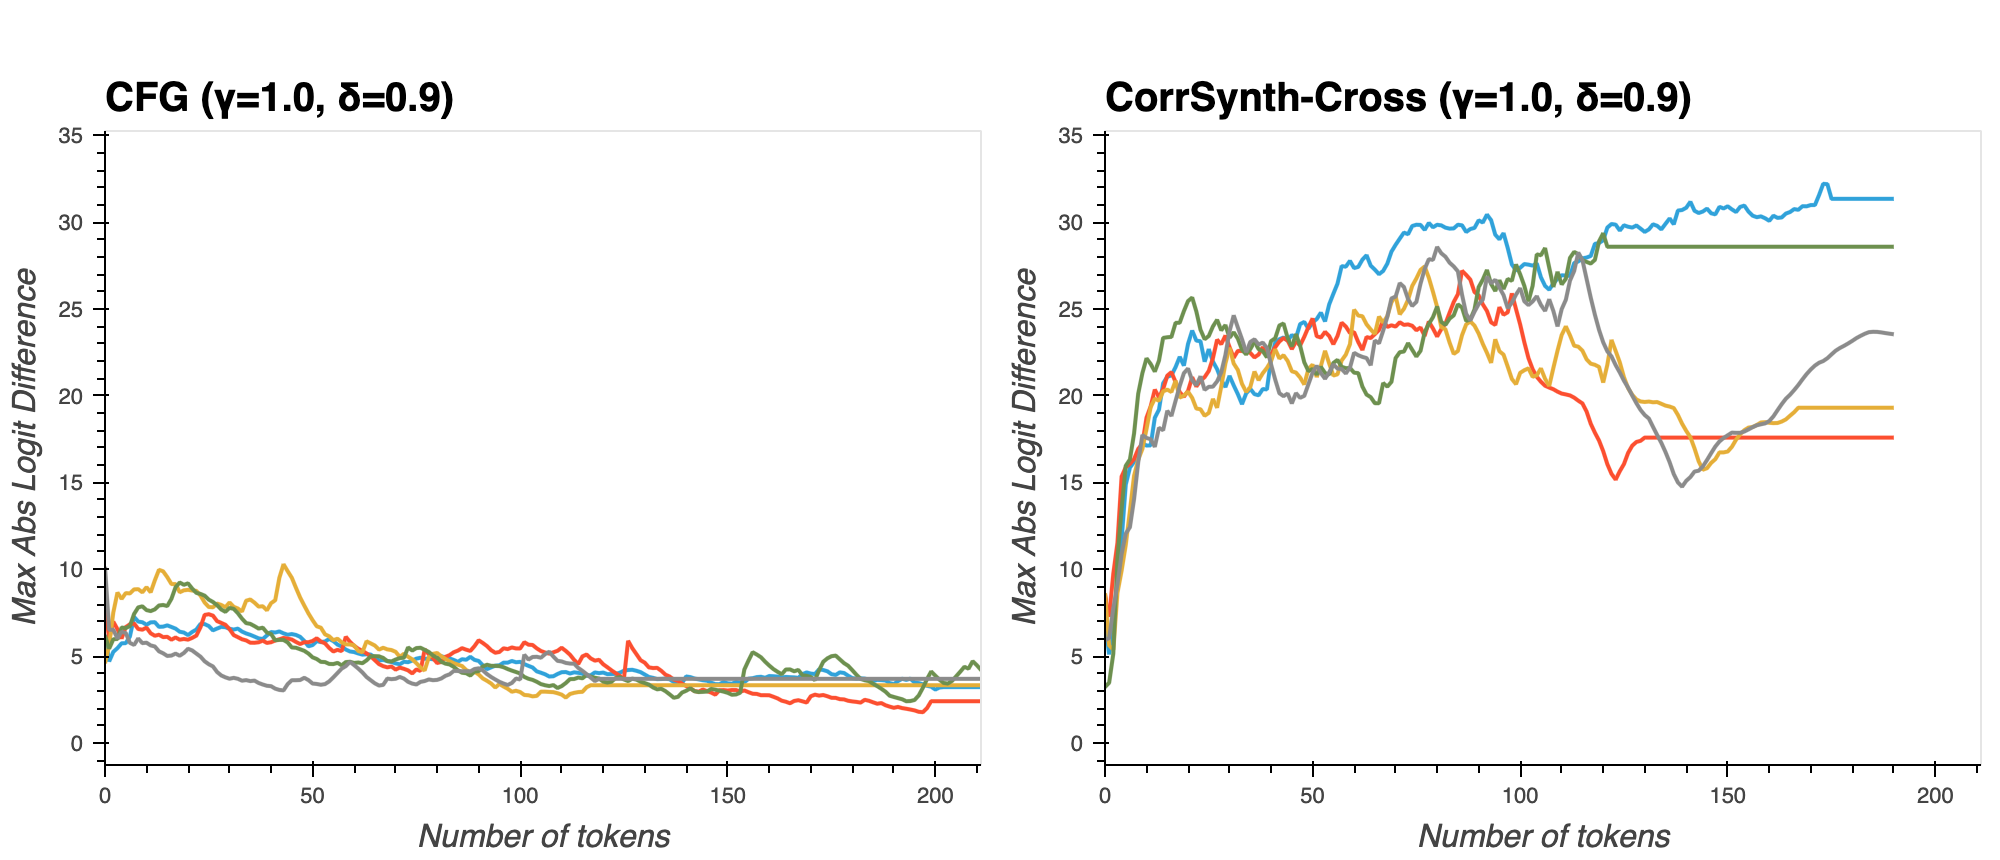
\includegraphics[width=0.5\textwidth]{figure/cfg_vs_corr.png}
\vspace{-0.8cm}
\caption{Generation progression from CFG and \corrsyn. We sample five generations using 3-shot prompts from \IMDb. The colored lines represent the absolute difference between logits of the current generation and contrast for each generation timestep (taken as an exponential moving average).}
\vspace{-1em}
\label{fig:cfg_vs_corrsynth}
\end{figure}


% \Category{}~\cite{blitzer-etal-2007-biographies} has Amazon product reviews and categories where the goal is to classify reviews into 23 categories, and hence in synthesis, we want to generate reviews for each of the categories. \Polarity~\cite{ni2019justifying} is Amazon product reviews dataset with positive and negative sentiment labels where the generation task involves asking the LLM to generate either a positive or a negative review for a a product. We do not provide any particular product to the LLM apart from those implicitly present in ICL examples. \Humor{} is a dataset about humorous and non-humorous questions about products. For generation, the label humorous or non-humorous is provided and the LLM is tasked to generate a corresponding question for any product on Amazon.



% \paragraph{Corpus.} In order to compare our results against \ours{} \citep{divekar2024synthesizrr} which uses retrieval-augmented generation for dataset synthesis, we use the five corpora mentioned in \autoref{tab:corpus} as the retrieval corpus. \RealNewsDom{} and \RealNewsInd{} are splits of news corpus \RealNews{} \citep{zellers2019grover}, which were filtered based by the country-headquarters of the news website \citep{divekar2024synthesizrr}. \Products{} contains metadata of products sold on e-commerce website Amazon \citep{ni-etal-2019-justifying}. Whereas \YelpCorpus{} corpus \cite{yelpcorpus} contains details of brick-and-mortar businesses listed on Yelp.com. \CMUMoviesCorpusShort{} corpus \cite{bamman-etal-2013-learning} contains 42k movie plot summaries. 

\paragraph{Teachers and students.} \ad{TODO fix this to be Mixtral. Cite.} As a teacher model, we use a frozen \Mixtral\ (8x7B) \citep{jiang2024mixtral} or \PhiMini\ (3.8B) \citep{abdin2024phi} for the data generation step. Following \citep{divekar2024synthesizrr}, we select examples randomly from the train set: 50 ICL examples per class for multi-class and 100 per class for binary. We think that this is a reasonable number of labeled examples since we are trading off the effort of labeling versus developing a potential zeroshot technique (which may not work well in practice). We use \DistilBERT{} student model (66M params \citet{Sanh2019DistilBERT}) as it is popular in prior work.

% Please add the following required packages to your document preamble:
% \usepackage{booktabs}
% \usepackage{multirow}
\begin{table*}[h]
\centering
\setlength{\tabcolsep}{3pt}
\begin{tabular}{
L{95pt}
% h
c % Teacher
c % C{16pt} % AG Accuracy
c % C{26pt} % IMDb Accuracy
c % C{16pt} % AG Mauve
c % C{26pt} % IMDb Mauve
c % C{16pt} % AG Self-BLEU-5
c % C{26pt} % IMDb Self-BLEU-5
c % C{16pt} % AG Entity Entropy
c % C{20pt} % IMDb Entity Entropy
}

\toprule
\multirow{2}{*}{\textbf{Method}}   
& \multirow{2}{*}{\textbf{Teacher}} %\multicolumn{1}{h}{\multirow{2}{*}{\textbf{Params}}}
% &  %\multicolumn{1}{C{26pt}}{\multirow{2}{*}{\textbf{Teacher}}}
& \multicolumn{2}{c}{\textbf{Accuracy}}
& \multicolumn{2}{c}{\textbf{MAUVE}}
& \multicolumn{2}{c}{\textbf{Self-BLEU-5}}
& \multicolumn{2}{c}{\textbf{Entity-Entropy}}
\\ 
\cmidrule(l){3-4}
\cmidrule(l){5-6}
\cmidrule(l){7-8}
\cmidrule(l){9-10} 
& \textbf{LM} % \multicolumn{1}{c}{\textbf{LM}}
& \textbf{{ } \AG} % AG Accuracy
& \textbf{\IMDb { }} % IMDb Accuracy
& \textbf{{ } \AG} % AG Mauve
& \textbf{\IMDb { }} % IMDb Mauve
& \textbf{{ } \AG} % AG Self-BLEU-5
& \textbf{\IMDb { }} % IMDb Self-BLEU-5
& \textbf{{ } \AG} % AG Entity Entropy
& \textbf{\IMDb { }} % IMDb Entity Entropy
\\ 
\midrule
\gold          
& -
& 91.4 & 91.4
& -	 & -	
& 17.1 & 27.9
& 6.6 & 7.5
\\ 
\midrule
%% 
%%
%%
\multicolumn{10}{c}{\underline{\textsc{Retrieval-based methods}}}  \\
\ReGen  
& \BERT
& 82.7 & $\otimes$
& 68.1 & $\otimes$
& 56.5 & $\otimes$
& \textbf{8.1 }& $\otimes$
\\ 
\SynthesizRR
& \LLaMa
& 84.6 & 84.8	
& \textbf{92.6} & 72.6	
& 34.2 & 62.9	
& 7.2 & 5.7
\\
\midrule 
%% 
%%
%%
\multicolumn{10}{c}{\underline{\textsc{Non-retrieval methods}}}  \\
\SunGen
& \GPTTwoXL
& $\otimes$ & 84.9	
& $\otimes$ & 68.7	
& $\otimes$ & \textbf{15.4}	
& $\otimes$ & 4.9
\\ 
\LetsSynth
& \ChatGPTShort
& $\otimes$ & \textbf{87.1}	
& $\otimes$ & 62.0	
& $\otimes$ & 62.2	
& $\otimes$ & 5.7
\\ 
\AttrPrompt
& \ChatGPTShort
& 79.8	& $\otimes$	
& 52.8	& $\otimes$	
& 39.8	& $\otimes$	
& 6.0	& $\otimes$
\vspace{1.5ex} 
\\ 
% \midrule 
% \multicolumn{10}{c}{\underline{\textsc{Ours}}}  \\
(Ours) \corrsynreallyshort-Intra
& \textsc{Phi-3 Mini}
& 84.8 & \textbf{87.1}
& 82.3 & \textbf{77.4}	
& 13.1 & 24.9	
& 7.4 & \textbf{6.5}
\\ 
(Ours) \corrsynreallyshort-Hybrid 
& \textsc{Phi-3 Mini}
& \textbf{85.1} & 86.8	
& 77.5 & 71.0	
& \textbf{12.1} & 19.2	
& 7.4 & 6.4
\\
\bottomrule
\end{tabular}
\caption{
Comparison of quality metrics and \DistilBERT\ student model fine-tuned on 6k rows from each approach. Mean accuracy across 5 training runs is considered. $\otimes$ indicates datasets were not released by authors.
}
\vspace{-1em}
\label{tab:baselines}
\end{table*}


\paragraph{Evaluation criteria} The task of evaluation of quality of text generation is quite challenging~\citep{llm-eval-survey}. Following prior works like \cite{divekar2024synthesizrr}, we evaluate synthetic generations based on several metrics. \textbf{Self-BLEU} \citep{bleu,zhu2018texygen} measures lexical diversity of a corpus of texts based on $n$-gram overlap between pairs of examples. \textbf{Entity entropy} measures the \textit{diversity} of entities in the generated texts using the distribution of each of 16 entity-types (inferred from a pre-trained named entity recognition model). Dataset which have high occurrence of few popular entities score lower on entropy. \textbf{MAUVE} \citep{liu-etal:divergence:neurips2021} measures closeness to human-written text using representations from a pre-trained \GPTTwoXL{} model. We also measure the \textbf{student accuracy} when trained on the synthetic data. We do not consider label preservation accuracy as it is susceptible to easy examples \cite{divekar2024synthesizrr}. In order to analyse the behavior of our strategy, we also study the label-wise cosine similarity of the generations, low dimensional embeddings of the generations using UMAP~\cite{mcinnes2020umap} and dataset cartography~\cite{swayamdipta-etal-2020-dataset}. %In addition, we also plot the visualizations of text representations of our generations against the \fewgen{} baseline as well (Section \ref{sec:analysis}).

\paragraph{Remark on diversity} In this work we are concerned about diversity at a dataset level and not an an instance level. To illustrate the difference between these two, consider the task of generating a long story. Here, it is important to ensure that the generated story has many of the features of a human written story (like complex storyline, many characters, non-repeating scenes etc.). But notice that ensuring such an instance level diversity does not guarantee diverse dataset of stories: multiple such stories obtained from an LLM could have a lot of overlap in content. For synthesis of good classification datasets, we require a more global notion of diversity which is at the dataset level. 

% In \S\ref{sec:student} we measure the effectiveness of synthetic data for student distillation. Besides the final performance of the student model, we also consider \textbf{label preservation accuracy}, the fraction of synthetic examples which are classified into prompted target class by an existing ``oracle'' model for the task. We construct the oracle by running a grid-search over \DeBERTaLarge{} hyperparams, splitting 80\% of the \gold{} train set for fine-tuning and 20\% for validation. %This metric is imperfect; it is possible to obtain very high label-preservation from a synthesis procedure generating easy-to-classify examples. These are of limited use for student generalization. Thus, we measure the training dynamics from the \textbf{Data Maps} generated by a \DistilBERT{} training run \citep{swayamdipta-etal-2020-dataset}. This identifies easy-to-learn, ambiguous and hard-to-learn synthetic examples.\gd{maybe revise or de-emphasize based on the final results}


\section{Results}
\label{sec:expts}

\subsection{Comparison to CFG}
We compare the effect of contrast as next-token generation proceeds in CFG and \corrsyn{}. To this end, we consider \IMDb{}, and sample continuations for five 3-shot prompts from both CFG and \corrsyn{} for the same Cross-label parameters: \mbox{$\{R=1, \gamma=1.0, \delta=0.9, \alpha=0\}$}. For each token, we store the maximum absolute difference of the current label logits vector and the contrast label logits vector (i.e. $\infty$-norm of logits difference of numerator and denominator in \eqref{eq:2corr_eq1} for \corrsyn{}, and similar terms in CFG). We plot this difference against the tokens generated. 

\autoref{fig:cfg_vs_corrsynth} shows the difference between CFG and \corrsyn{}: as token generation proceeds, the effect of contrast in CFG is muted. This happens since the same generated sequence for the current label is fed back into the contrast model and thus the effect of the contrastive prompt reduces over later token generations. Whereas in \corrsyn{}, the effect of the guidance or contrast persists. As a result, we believe \corrsyn{} is a better suited for longer generations where guidance is required for the entirety of generation. In terms of complexity, as discussed previously, we incur a much higher complexity of LLM model forward passes in CFG (detailed comparison in \aref{app:compute_complexity}). 


\subsection{Comparison to \fewgen}
\label{sec:corrsyn_results}
In this section, we present our experimental results against \fewgen. We use the following settings:

\insection[:]{\corrsyn{} Cross-label} Repeat factor $R=1$, Uniform contrastive guidance with \mbox{$\gamma=1.0 $} and $\delta=0.9\times\gamma$ and plausibility criterion $\alpha=10^{-3}$.

\insection[:]{\corrsyn{} Intra-label} Repeat factor $R=2$, Uniform contrastive guidance with \mbox{$\gamma=1.0 $} and $\delta=0.5\times\gamma$ and plausibility criterion $\alpha=10^{-3}$.

\insection[:]{\corrsyn{} Hybrid} Repeat factor $R=2$, set $\gamma=1.0$, Set $\gamma_{intra}=\gamma/2$, $\gamma_{cross}=\gamma/10$. Then uniform contrastive guidance in each of intra and cross terms. We set plausibility criterion \mbox{$\alpha=10^{-3}$}.
% \begin{itemize}
%     \item Cross-label \corrsyn\
%     \begin{itemize}
%         \item Repeat factor $R=1$
%         \item Uniform contrastive guidance with \mbox{$\gamma\in\{0.5,1.0,1.5\}$} and $\delta=0.9\times\gamma$
%         \item Plausibility criterion $\alpha=10^{-3}$
%     \end{itemize}
%     \item Hybrid \corrsyn\
%     \begin{itemize}
%         \item Set repeat factor $R=2$. 
%         \item Set $\gamma_{intra}=$, $\gamma_{cross}=$. Use uniform contrastive guidance within intra and cross contrasts: for intra, we set $\gamma_{m,n}=\frac{\gamma_{intra}}{R-1}$, and for cross $\gamma_{m,n}=\frac{\gamma_{cross}}{(K-1)R}$ where $K$ is the number of classes. 
%         \item Plausibility constraint $\alpha=10^{-3}$
%     \end{itemize}
% \end{itemize}


We observe in \autoref{tab:accuracy-diversity-icl} that 3-shot \corrsyn{} outperforms \fewgen{} on all evaluation metrics. Specifically, using Hybrid and Intra variants, we can achieve better student model accuracy (\DistilBERT) while increasing diversity (lower Self-BLEU, higher entity entropy) and better match with human-written text (better MAUVE). For MAUVE computation, we have used embeddings based on a GPT-2XL model. We have only shown the results for Intra and Hybrid variants since from our ablations they performed best. In \autoref{app:zeroshot}, we note the zero-shot results, which demonstrate comparable gains on all metrics. 





\begin{figure*}[!t] % Use figure* to span both columns
    \centering
    \begin{subfigure}[t]{\textwidth}
        \centering
        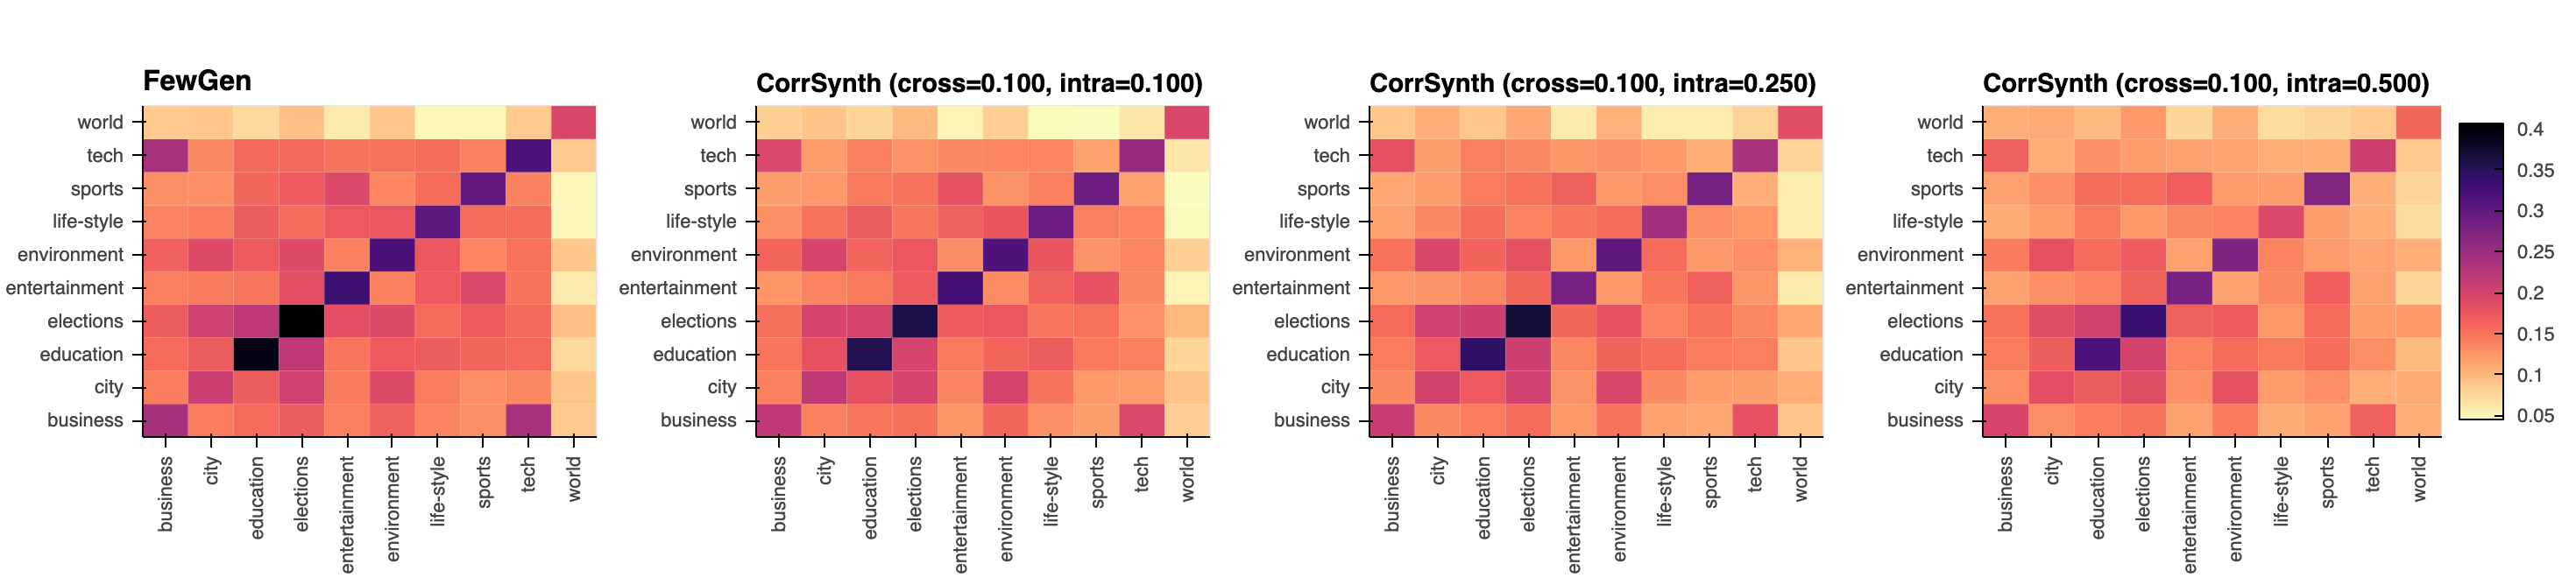
\includegraphics[width=\textwidth]{figure/cosine_intra_variation_v2.png}
        \caption{Impact of increasing Intra-label contrast (left to right) in Hybrid \corrsyn\ upon label-wise cosine similarities.}
        \label{fig:cosine_intra}
    \end{subfigure}
    \vskip\baselineskip
    \vspace{-0.7cm}
    \begin{subfigure}[t]{\textwidth}
        \centering
        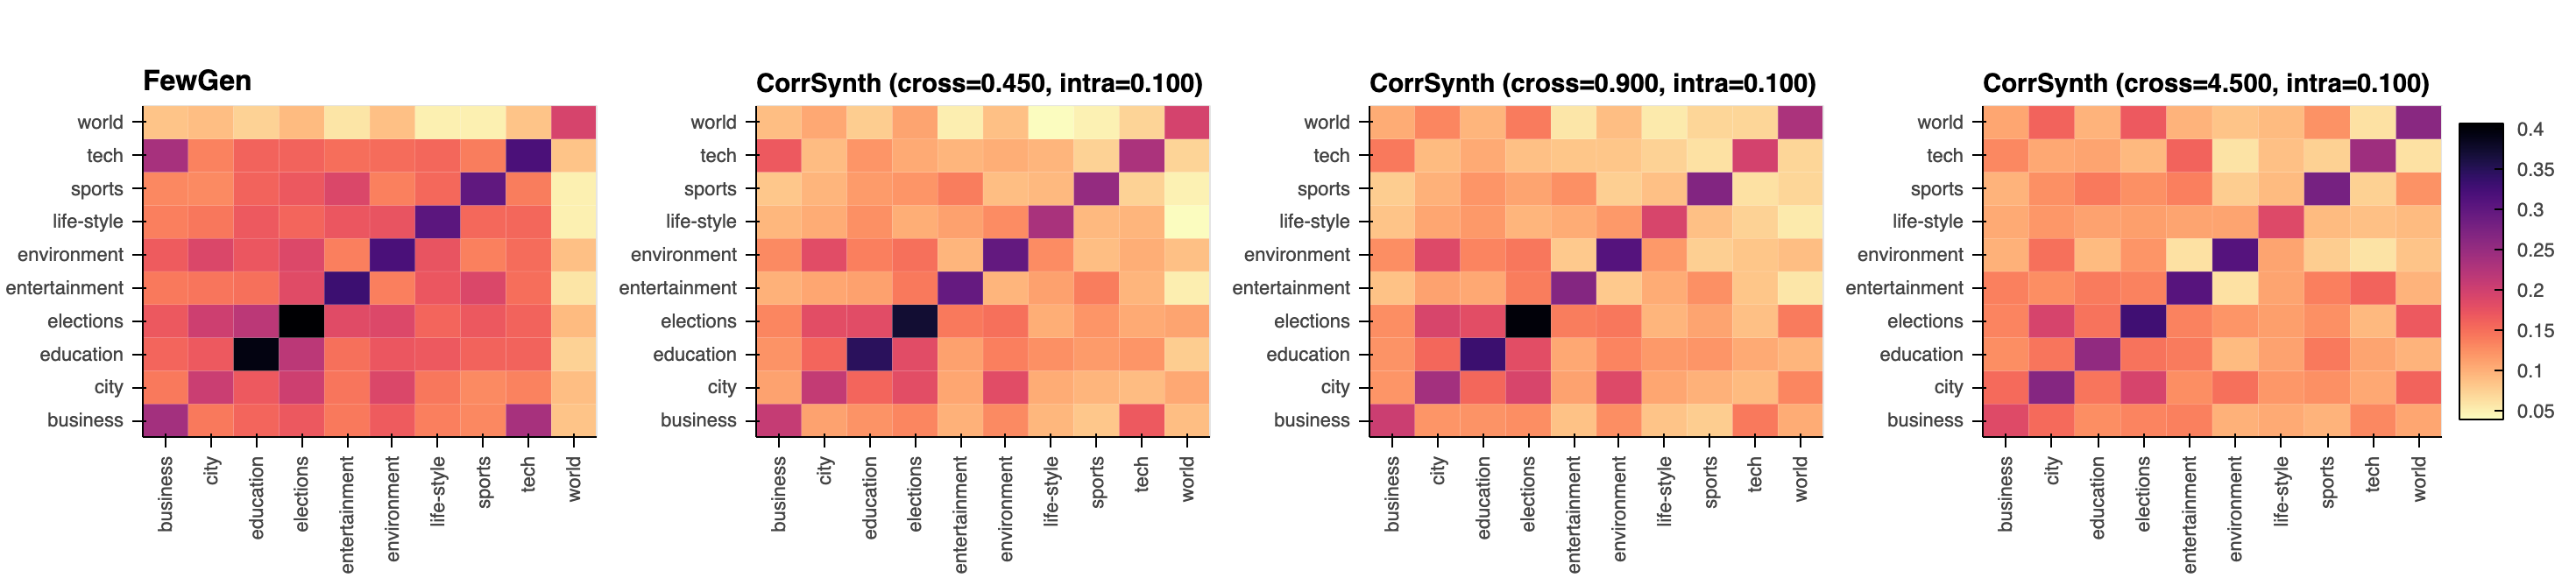
\includegraphics[width=\textwidth]{figure/cosine_cross_variation_v2.png}
        \caption{Impact of increasing Cross-label contrast (left to right) in Hybrid \corrsyn\ upon label-wise cosine similarities.}
        \label{fig:cosine_cross}
    \end{subfigure}
    \caption{Heatmaps for label-wise cosine similarities on \ToIHeadlines\ (with Phi-3-mini) as we increase Intra-label contrast vs increasing cross-label contrast. Note that ``Cross'' and ``Intra'' in figure titles correspond to $\gamma_{cross}$ and $\gamma_{intra}$ respectively. \fewgen\ heatmaps are provided for reference.}
    \vspace{-1em}
    \label{fig:cosine}
\end{figure*}





\subsection{Comparison to prior works} 

In \autoref{tab:baselines} we compare \corrsyn{} to current dataset generation methods as baselines. Baseline numbers are quoted from \citet{divekar2024synthesizrr}, where all results are reported on 6k rows using \DistilBERT\ student (same as our setup). The following SOTA generation methods have been compared: 
(1) \textbf{\ReGen{}} \cite{yu-etal-2023-regen}: uses dual BERT models - one for retrieval and one as a classifier - to perform multi-round filtering and eliminate noisy data based on model consistency; 
(2) \textbf{\SynthesizRR{}} \cite{divekar2024synthesizrr}: develops a hybrid retrieval-augmentation based approach to rewrite contexts, greatly enhancing the diversity of generated text;
(3) \textbf{\SunGen{}} \cite{gao2023selfguided}: employs \ZeroGen{} \cite{ye2022zerogen} to create a substantial synthetic dataset (200k rows) and then uses a bi-level optimization algorithm to assign instance-weights to each synthetic example; 
(4) \textbf{\LetsSynth{}} \cite{wang-etal-2023-lets}: builds a distinct ``seed dataset'' to train a student model, leverages an LLM to identify errors, and synthesizes supplementary data. This cycle of data augmentation is repeated.
(5) \textbf{\AttrPrompt{}} \cite{yu2023large}: enhances dataset diversity and unbiasedness by prompting a potent LLM like \ChatGPT{} with attributes identified through human-in-the-loop task analysis.

We divide our comparison into non-retrieval and retrieval based synthesis, as the latter naturally demonstrates higher diversity \citep{divekar2024synthesizrr}. We observe that \corrsyn{} achieves strong performance on all metrics, despite using a small teacher LLM (\PhiMini with 3.8B parameters) compared to prior approaches. 




\begin{figure*}[!t]
\centering
    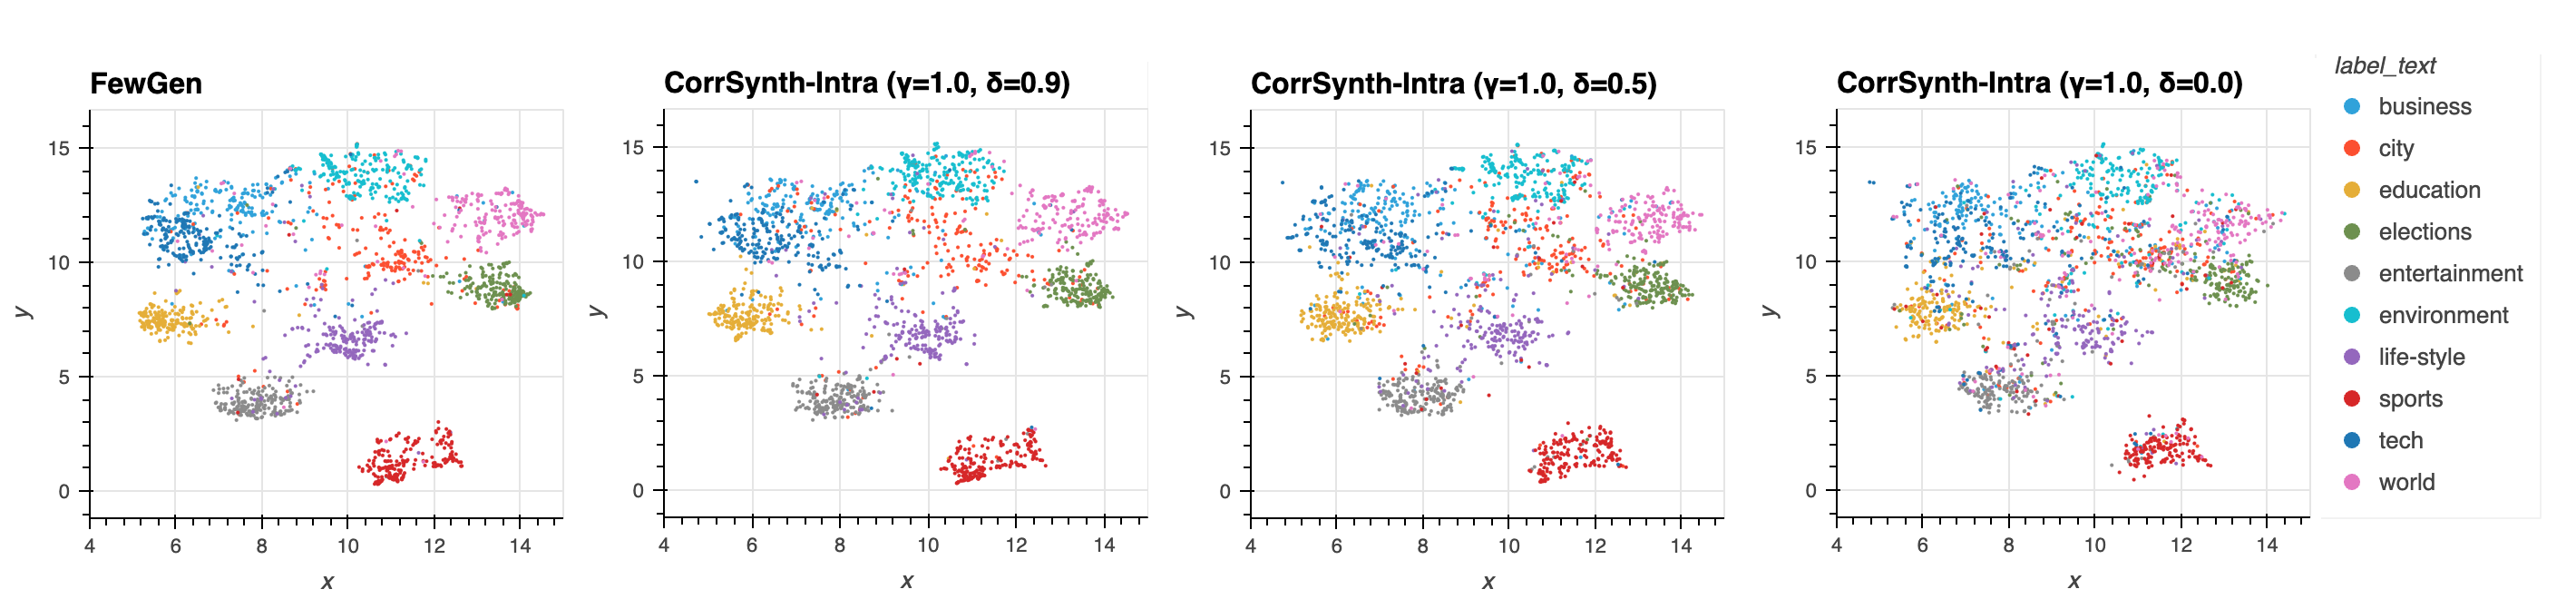
\includegraphics[width=\textwidth]{figure/umaps_v3.png}
    \vspace{-0.8cm}
    \caption{Visualising two-dimensional text representations of generations (on \ToIHeadlines\ with \PhiMini) using \corrsyn-Intra. We gradually increase guidance delta, $\delta$ in $(0.0, 0.5, 0.9)$. \fewgen\ plot is provided as a reference to the unmodified clusters (it is equivalent to $\delta=1$ i.e. no contrast).}
    \vspace{-1em}
    \label{fig:intra_label_umaps}
\end{figure*}





%Additional intrinsic analysis in \autoref{ta:bmauve} shows that the generations from \corrsyn{} more closely match human-written text in terms of Mauve (which generates embeddings based on a GPT-2XL model). Thus we are able to achieve much more realistic text through our approach. 
% \ad{Merge MAUVE with main results table}



% % Please add the following required packages to your document preamble:
% % \usepackage{booktabs}
% % \usepackage{multirow}
% \begin{table*}[h]
% \centering
% \begin{tabular}{
% L{18pt}
% C{18pt}
% C{18pt}
% C{18pt}
% C{18pt}
% C{18pt}
% C{18pt}
% C{18pt}
% C{18pt}
% }
% \toprule
% \multicolumn{1}{l}{\multirow{2}{*}{\textbf{Method}}} & \multicolumn{1}{c}{\multirow{2}{*}{\textbf{Source}}} & \multicolumn{1}{c|}{\multirow{2}{*}{\textbf{Teacher LM}}} & \multicolumn{3}{c|}{\textbf{Sentiment}}                    & \multicolumn{3}{c}{\textbf{Topic}}                            \\ 

% \cmidrule(l){2-7} 

% \multicolumn{1}{l|}{}                     & \textbf{\Pol} & \textbf{\Yelp} & \multicolumn{1}{c|}{\textbf{\IMDb}} & \textbf{\AG} & \textbf{\ToI} & \textbf{\Cat} \\ \midrule
% \multicolumn{1}{l|}{\gold}                 & 0     & 0             & \multicolumn{1}{c|}{0}             & 0    & 0          & 0                 \\ \midrule
% \multicolumn{7}{c}{\underline{\textsc{Zero-shot}}}                                                                                                                                                         \\
% \multicolumn{1}{l|}{\AttrPrompt}           & 0     & 0             & \multicolumn{1}{c|}{0}             & 0    & 0          & 0                 \\
% \multicolumn{1}{l|}{\fewgen}               & 0     & 0             & \multicolumn{1}{c|}{0}             & 0    & 0          & 0                 \\
% \multicolumn{1}{l|}{\ours}          & 0     & 0             & \multicolumn{1}{c|}{0}             & 0    & 0          & 0                 \\
% \multicolumn{1}{l|}{\corrsyn}            & 0     & 0             & \multicolumn{1}{c|}{0}             & 0    & 0          & 0                 \\ \midrule
% \multicolumn{7}{c}{\underline{\textsc{Few-shot (Human seed)}}}                                                                                                                                             \\
% \multicolumn{1}{l|}{\Human\ ICL + \fewgen}    & 0     & 0             & \multicolumn{1}{c|}{0}             & 0    & 0          & 0                 \\
% \multicolumn{1}{l|}{\Human\ ICL + \oursshort}      & 0     & 0             & \multicolumn{1}{c|}{0}             & 0    & 0          & 0                 \\
% \multicolumn{1}{l|}{\Human\ ICL + \corrsyn}             & 0     & 0             & \multicolumn{1}{c|}{0}             & 0    & 0          & 0                 \\ \midrule
% \multicolumn{7}{c}{\underline{\textsc{Few-shot (Generated seed)}}}                                                                                                                                         \\
% \multicolumn{1}{l|}{\fewgen\ ICL + \fewgen}            & 0     & 0             & \multicolumn{1}{c|}{0}             & 0    & 0          & 0                 \\
% \multicolumn{1}{l|}{\fewgen\ ICL + \oursshort}     & 0     & 0             & \multicolumn{1}{c|}{0}             & 0    & 0          & 0                 \\
% \multicolumn{1}{l|}{\corrsyn\ ICL + \fewgen}            & 0     & 0             & \multicolumn{1}{c|}{0}             & 0    & 0          & 0                 \\
% \multicolumn{1}{l|}{\corrsyn\ ICL + \oursshort}  & 0     & 0             & \multicolumn{1}{c|}{0}             & 0    & 0          & 0                 \\ \bottomrule
% \end{tabular}
% \caption{Performance comparison of student model (DistilBERT) fine-tuned on generated datasets on each method. We report mean accuracy numbers across 5 runs (The standard deviation across the runs was $<0.5$, hence, we do not report it.)}
% \end{table*}






% % % Please add the following required packages to your document preamble:
% % \usepackage{booktabs}
% % \usepackage{multirow}
% \begin{table}[]
% \small
% \centering
% \begin{tabular}{
% L{38pt}
% C{16pt} 
% C{16pt}
% C{20pt} |
% C{16pt}
% C{16pt}
% C{16pt}
% }
% \toprule
% \multirow{2}{*}{\textbf{Method}} 
% & \multicolumn{3}{c|}{\textbf{Sentiment}}      
% & \multicolumn{3}{c}{\textbf{Topic}}        
% \\ 
% \cmidrule(l){2-7} 
% & \textbf{\Pol} 
% & \textbf{\Yelp} 
% & \textbf{\IMDb} 
% & \textbf{\AG} 
% & \textbf{\ToI} 
% & \textbf{\Cat} 
% \\ \midrule
% % \gold             
% % & 0            & 0             & 0             & 0           & 0            & 0            \\
% \AttrPromptShort             
% & -            & 55.9          & -          & 52.8      & -            & -            \\
% \fewgen             
% & 65.2         & 80.4          & 60.8       & 78.4      & 67.8         & 64.1         \\
% \oursshort            
% & -            & 76.6          & 60.3       & 94.0      & 71.7         & 65.0         \\ 
% \corrsynshort             
% & 71.8         & 85.5          & 66.9       & 86.2      & 74.9         & -            \\ 
% \bottomrule
% \end{tabular}
% \caption{Mauve results (3-shot Human-annotated ICL set). Synthesis results are generated from \textsc{Mistral-7B-Instruct} teacher LM.}
% \label{tab:mauve}
% \end{table}


% \begin{table}[h]
% \centering
% \sisetup{round-mode=places, round-precision=1} % Set the rounding precision
% \setlength{\tabcolsep}{1.9pt}
% \footnotesize{
% \scalebox{0.9}{
% \begin{tabular}{
% C{1.65cm}  % Method
% C{1.45cm}  % Teacher LM
% C{2.7cm}  % Retriever
% c % S[table-format=3.2]  % Yelp Self-BLEU
% c % S[table-format=3.2]  % AG News Self-BLEU
% c % S[table-format=3.2]  % IMDb Self-BLEU
% c % S[table-format=3.2]  % SST-2 Self-BLEU
% % c 
% |c % S[table-format=3.2]  % Yelp Entity Entropy
% c % S[table-format=3.2]  % AG News Entity Entropy
% c % S[table-format=3.2]  % IMDb Entity Entropy
% c  % S[table-format=3.2]  % SST-2 Entity Entropy
% % c 
% |c % S[table-format=3.2]  % Yelp Mauve
% c % S[table-format=3.2]  % AG News Mauve
% c % S[table-format=3.2]  % IMDb Mauve
% c % S[table-format=3.2]  % SST-2 Mauve
% }
% \toprule
% % \multirow{3}{*}{\textbf{Method}}
% % & \multirow{3}{*}{ \textbf{Student LM} }
% % & \multicolumn{1}{c}{\underline{\RNInd}} 
% % & \multicolumn{2}{c}{\underline{\RNDom}} 
% % & \multicolumn{3}{c}{\underline{\Products}} 
% % & \multirow{3}{*}{\textbf{Avg}}
% % \\
% % [0.5ex]
% \textbf{Method}
% & \textbf{Teacher}
% & \multirow{2}{*}{\textbf{Params}}
% & \multicolumn{4}{c}{\underline{Self-BLEU-5 \lowerbetter}} 
% % &
% & \multicolumn{4}{c}{\underline{Entity Entropy \higherbetter}} 
% % &
% & \multicolumn{4}{c}{\underline{Mauve \higherbetter}} 
% \\
% [0.7ex]
% \textit{(Dataset)}
% & \textbf{LM}
% & 
% & \AG % Self-BLEU
% & \ToI % Self-BLEU
% & \Pol % Self-BLEU
% & \Hum % Self-BLEU
% % & 
% & \AG % Self-BLEU
% & \ToI % Self-BLEU
% & \Pol % Self-BLEU
% & \Hum % Self-BLEU
% % & 
% & \AG % Self-BLEU
% & \ToI % Self-BLEU
% & \Pol % Self-BLEU
% & \Hum % Self-BLEU
% \\ 
% \midrule
%  \gold &  - & - 
%  & 11.3  &  5.9  & 14.4   &  15.0 
%  & 5.8   & 5.3   &  6.0  &  3.9 
%  &  -  &  -  &  -  & -   
%  \vspace{0.75ex} \\ 

%  \toprule
% \multicolumn{15}{c}{\underline{\textsc{3- shot}}} \vspace{1ex} \\
% \fewgen &  \LLaMa & \_ &  23.6  &  18.5  &  50.5  &  36.8  &  5.5  &  5.0  &  3.8  &  3.2  &  96.5  &  97.7  &  81.9  &  94.2 \\
%  \corrsyn &  \LLaMa & $\gamma=0.5, \delta=0.45$ 
%  &  \best{6.4}  &  \best{6.0}  &  \best{7.4}  &  \best{10.1}  
%  &  6.0  &  \best{5.3}  &  5.6  &  \best{4.0} 
%  &  96.2  &  98.2  &  \best{90.6}  &  \best{99.7}  \\
%  \corrsyn &  \LLaMa & $\gamma=0.5, \delta=0.5$ 
%  &  6.7  &  6.4  & 7.9  &  10.7  
%  &  \best{6.1}  &  5.2  &  \best{5.7}  &  3.9  
%  &  95.8  &  98.0  &  88.1  &  \best{99.7}  \\
%  \corrsyn &  \LLaMa & $\gamma=1.0, \delta=0.9$ 
% & 20.8  &  14.4  & 43.9   &  30.1  
%  & 5.5   & 4.9   &  3.8  &  3.0
%  & \best{96.7}   &  \best{98.8}  &  82.1  & 96.1   \\
%  \corrsyn &  \LLaMa & $\gamma=1.0, \delta=1.0$ 
%  & 22.4  &  17.9  & 48.6   &  32.7  
%  & 5.6   & 5.0   &  4.1  &  2.9
%  &  96.4  &  98.7  &  80.1  & 94.6   \\
%   \corrsyn &  \LLaMa & $\gamma=1.5, \delta=1.35$ 
%  & 37.4  &  30.9  & 67.8   &  54.4  
%  & 5.1   & 4.6   &  3.1  &  2.8
%  &  94.6  &  98.0  &  72.2  & 91.9   \\
%   \corrsyn &  \LLaMa & $\gamma=1.5, \delta=1.5$ 
%  & 40.2  &  35.1  & 70.3   &  59.7  
%  & 5.5   & 4.4   &  2.9  &  2.5
%  &  91.4  &  97.7  &  70.4  & 88.6   \\
% [0.75ex]
% \bottomrule
% \end{tabular}
% }
% }
% \caption{
% Intrinsic evaluations of synthetic datasets generated by \fewgen\ and \corrsyn. We also compare against the gold dataset. We subsample all to 2k examples before computing metrics. Within each dataset, we \textbf{bold} the best result.
% }
% \vspace{-3ex}
% \label{tab:baselines-intrinsic}
% \end{table}



% \section{Ablations}
% \label{sec:ablations}
% In this section we provide our ablation results. We measure the variation of \textbf{Self-BLEU}, \textbf{Entity entropy}, \textbf{MAUVE} and \textbf{student accuracy} as we vary each parameter by keeping others fixed. In particular we vary i) guidance $\gamma\in \{0.1,0.5,1.0,1.5,3,10\}$\sk{what is the final grid for gamma}, ii) $\delta\in\{0,1.0,0.5\gamma,0.95\gamma,\gamma,1.05\gamma,\}$\sk{what is the final grid for delta?}, iii) repeat factor $R\in\{1,3\}$, iv) contrast type in cross-label v/s hybrid\sk{rewrite hybrid, by removing ration}



% % Please add the following required packages to your document preamble:
% % \usepackage{booktabs}
% \begin{table}[]\small
% \centering
% \begin{tabular}{@{}lccccc@{}}
% \toprule
% \textbf{Method} & \textbf{Params} & \AGNews    & \ToI  & \Polarity & \Humor \\ \midrule
% \gold            & \_              & 88.78          & 75.08         & 89.68             & 91.56          \\ \midrule
% \fewgen          & \_              & 84.08          & 69.96         & 86.34             & 86.74          \\
% \corrsyn            & $\gamma=0.5, \delta=0.45$              & 84.47          & \textbf{72.2} & 88.26             & \textbf{88.00} \\
% \corrsyn            & $\gamma=0.5, \delta=0.5$              & 84.43          & 70.68         & \textbf{88.60}    & 87.05          \\
% \corrsyn            & $\gamma=1.0, \delta=0.9$              & 83.76          & 69.33         & 86.39             & 87.62          \\
% \corrsyn            & $\gamma=1.0, \delta=1.0$              & 84.16          & 68.72         & 85.75             & 86.81          \\
% \corrsyn            & $\gamma=1.5, \delta=1.35$              & \textbf{84.59} & 70.06         & 84.59             & 86.16          \\
% \corrsyn            & $\gamma=1.5, \delta=1.5$              & 84.17          & 68.31         & 85.71             & 85.13          \\ \bottomrule
% \end{tabular}
% \caption{Performance comparison of student model (DistilBERT) fine-tuned on generated datasets on each method. We report mean accuracy numbers across 5 runs (The standard deviation across the runs was $<0.5$, hence, we do not report it.)}
% \end{table}



% \begin{table}[!h]
% \centering
% \sisetup{round-mode=places, round-precision=1} % Set the rounding precision
% \setlength{\tabcolsep}{2pt}
% \footnotesize{
% \begin{tabular}{
% l
% c
% h % L{2.4cm}  % Student
% S[table-format=3.2]  % ToI
% S[table-format=3.2] S[table-format=3.2] % Realnews 
% S[table-format=3.2] S[table-format=3.2] S[table-format=3.2] % Products
% l  % Average
% }
% \toprule
% % \multirow{3}{*}{\textbf{Method}}
% % & \multirow{3}{*}{ \textbf{Student LM} }
% % & \multicolumn{1}{c}{\underline{\RNInd}} 
% % & \multicolumn{2}{c}{\underline{\RNDom}} 
% % & \multicolumn{3}{c}{\underline{\Products}} 
% % & \multirow{3}{*}{\textbf{Avg}}
% % \\
% % [0.5ex]
% \textbf{Method}
% & \multirow{2}{*}{\textbf{Teacher LM}}
% &  
% & \AG{}  
% & \Humor{} 
% & \Intent{} 
% & \multirow{2}{*}{\textbf{Avg}}
% \\
% \textit{(Dataset size)}
% & 
% & 
% & \text{($2$K)}
% & \text{($2$K)}
% & \text{($2$K)}
% &
% \\ 
% % &                   &         &         &         &         &         &  \\ 
% % \cmidrule{1-2}                        \cmidrule{3-5} \cmidrule{7-9}
% % [-0.5ex]
% \midrule
% \gold &
% % & \TinyBERT{}       &     77.83 &         87.9 &       81.23 &         70.41 &      89.22 &         87.09 & 82.28 \\
% % & \DistilBERT{}     &     82.16 &        90.45 &       88.92 &         78.44 &      91.69 &         90.78 & 87.07 \\
% & \DeBERTa{}         &   &   &   & 
% % \vspace{1ex}
% \\

% %  ____                 ___  _          _
% % |_  / ___  _ _  ___  / __|| |_   ___ | |_
% %  / / / -_)| '_|/ _ \ \__ \| ' \ / _ \|  _|
% % /___|\___||_|  \___/ |___/|_||_|\___/ \__|

% % \midrule
% % \vspace{2ex}
% \toprule
% % \multicolumn{6}{c}{\underline{\textsc{Zero shot}}} \vspace{1ex} \\
% % \fewgen & \LLaMa
% % & \TinyBERT{}        &  71.96 &  62.69 &  57.85 &    48.0 &  83.15 &  74.55 & 66.37 \\
% % & \DistilBERT{}      &  59.45 &  66.56 &  58.77 &  57.79 &  67.74 &  80.37 & 65.11 \\
% % & \DeBERTa{} &  49.82 &  64.45 &  70.46 &  57.25 &  70.31 &  87.69 & 66.66 \\
% % & \DeBERTa{} &   &   &   &
% % \\
% % [1ex] 

% % \midrule

% \corrsyn & \LLaMa 
% % & \TinyBERT{}        &  68.56 &  84.06 &  58.15 &   61.5 &  78.15 &  79.45 & 71.64 \\
% % & \DistilBERT{}      &  72.86 &  85.54 &   60.0 &  70.97 &  79.91 &  79.71 & 75.11 (74.83) \\
% % & \DeBERTa{} &  73.95 &  85.55 &  70.15 &  70.12 &  85.71 &  88.02 & 78.92 
% & \DeBERTa{} &  &   &   &
% \vspace{1.5ex}
% \\

% \toprule
% \multicolumn{6}{c}{\underline{\textsc{Few shot}}} \vspace{1ex} \\
% \fewgen & \LLaMa
% % & \TinyBERT{}        &  71.96 &  62.69 &  57.85 &    48.0 &  83.15 &  74.55 & 66.37 \\
% % & \DistilBERT{}      &  59.45 &  66.56 &  58.77 &  57.79 &  67.74 &  80.37 & 65.11 \\
% % & \DeBERTa{} &  49.82 &  64.45 &  70.46 &  57.25 &  70.31 &  87.69 & 66.66 \\
% & \DeBERTa{} &   &   &   &
% \\
% % [1ex] 

% % \midrule

% \corrsyn & \LLaMa 
% % & \TinyBERT{}        &  68.56 &  84.06 &  58.15 &   61.5 &  78.15 &  79.45 & 71.64 \\
% % & \DistilBERT{}      &  72.86 &  85.54 &   60.0 &  70.97 &  79.91 &  79.71 & 75.11 (74.83) \\
% % & \DeBERTa{} &  73.95 &  85.55 &  70.15 &  70.12 &  85.71 &  88.02 & 78.92 
% & \DeBERTa{} &  &   &   &
% \vspace{1.5ex}
% \\




                                
% \bottomrule
% \end{tabular}
% }
% \caption{Accuracy}
% \label{tab:student-deb}
% \end{table}



% \begin{table}[!h]
% \centering
% \sisetup{round-mode=places, round-precision=1} % Set the rounding precision
% \setlength{\tabcolsep}{2pt}
% \footnotesize{
% \begin{tabular}{
% l
% c
% h % L{2.4cm}  % Student
% S[table-format=3.2]  % ToI
% S[table-format=3.2] S[table-format=3.2] % Realnews 
% S[table-format=3.2] S[table-format=3.2] S[table-format=3.2] % Products
% l  % Average
% }
% \toprule
% % \multirow{3}{*}{\textbf{Method}}
% % & \multirow{3}{*}{ \textbf{Student LM} }
% % & \multicolumn{1}{c}{\underline{\RNInd}} 
% % & \multicolumn{2}{c}{\underline{\RNDom}} 
% % & \multicolumn{3}{c}{\underline{\Products}} 
% % & \multirow{3}{*}{\textbf{Avg}}
% % \\
% % [0.5ex]
% \textbf{Method}
% & \multirow{2}{*}{\textbf{Teacher LM}}
% &  
% & \AG{}  
% & \Humor{} 
% & \Intent{} 
% & \multirow{2}{*}{\textbf{Avg}}
% \\
% \textit{(Dataset size)}
% & 
% & 
% & \text{($2$K)}
% & \text{($2$K)}
% & \text{($2$K)}
% &
% \\ 
% % &                   &         &         &         &         &         &  \\ 
% % \cmidrule{1-2}                        \cmidrule{3-5} \cmidrule{7-9}
% % [-0.5ex]
% \midrule
% \gold &
% % & \TinyBERT{}       &     77.83 &         87.9 &       81.23 &         70.41 &      89.22 &         87.09 & 82.28 \\
% % & \DistilBERT{}     &     82.16 &        90.45 &       88.92 &         78.44 &      91.69 &         90.78 & 87.07 \\
% & \DeBERTa{}         &   &   &   & 
% % \vspace{1ex}
% \\

%  ____                 ___  _          _
% |_  / ___  _ _  ___  / __|| |_   ___ | |_
%  / / / -_)| '_|/ _ \ \__ \| ' \ / _ \|  _|
% /___|\___||_|  \___/ |___/|_||_|\___/ \__|

% \midrule
% \vspace{2ex}
% \toprule
% \multicolumn{6}{c}{\underline{\textsc{Zero shot}}} \vspace{1ex} \\
% \fewgen & \LLaMa
% % & \TinyBERT{}        &  71.96 &  62.69 &  57.85 &    48.0 &  83.15 &  74.55 & 66.37 \\
% % & \DistilBERT{}      &  59.45 &  66.56 &  58.77 &  57.79 &  67.74 &  80.37 & 65.11 \\
% % & \DeBERTa{} &  49.82 &  64.45 &  70.46 &  57.25 &  70.31 &  87.69 & 66.66 \\
% & \DeBERTa{} &   &   &   &
% \\
% % [1ex] 

% % \midrule

% \corrsyn & \LLaMa 
% % & \TinyBERT{}        &  68.56 &  84.06 &  58.15 &   61.5 &  78.15 &  79.45 & 71.64 \\
% % & \DistilBERT{}      &  72.86 &  85.54 &   60.0 &  70.97 &  79.91 &  79.71 & 75.11 (74.83) \\
% % & \DeBERTa{} &  73.95 &  85.55 &  70.15 &  70.12 &  85.71 &  88.02 & 78.92 
% & \DeBERTa{} &  &   &   &
% \vspace{1.5ex}
% \\

% \toprule
% \multicolumn{6}{c}{\underline{\textsc{Few shot}}} \vspace{1ex} \\
% \fewgen & \LLaMa
% % & \TinyBERT{}        &  71.96 &  62.69 &  57.85 &    48.0 &  83.15 &  74.55 & 66.37 \\
% % & \DistilBERT{}      &  59.45 &  66.56 &  58.77 &  57.79 &  67.74 &  80.37 & 65.11 \\
% % & \DeBERTa{} &  49.82 &  64.45 &  70.46 &  57.25 &  70.31 &  87.69 & 66.66 \\
% & \DeBERTa{} &   &   &   &
% \\
% % [1ex] 

% % \midrule

% \corrsyn & \LLaMa 
% % & \TinyBERT{}        &  68.56 &  84.06 &  58.15 &   61.5 &  78.15 &  79.45 & 71.64 \\
% % & \DistilBERT{}      &  72.86 &  85.54 &   60.0 &  70.97 &  79.91 &  79.71 & 75.11 (74.83) \\
% % & \DeBERTa{} &  73.95 &  85.55 &  70.15 &  70.12 &  85.71 &  88.02 & 78.92 
% & \DeBERTa{} &  &   &   &
% \vspace{1.5ex}
% \\




                                
% \bottomrule
% \end{tabular}
% }
% \caption{BLEU}
% \label{tab:student-deb}
% \end{table}



% \begin{table}[!h]
% \centering
% \sisetup{round-mode=places, round-precision=1} % Set the rounding precision
% \setlength{\tabcolsep}{2pt}
% \footnotesize{
% \begin{tabular}{
% l
% c
% h % L{2.4cm}  % Student
% S[table-format=3.2]  % ToI
% S[table-format=3.2] S[table-format=3.2] % Realnews 
% S[table-format=3.2] S[table-format=3.2] S[table-format=3.2] % Products
% l  % Average
% }
% \toprule
% % \multirow{3}{*}{\textbf{Method}}
% % & \multirow{3}{*}{ \textbf{Student LM} }
% % & \multicolumn{1}{c}{\underline{\RNInd}} 
% % & \multicolumn{2}{c}{\underline{\RNDom}} 
% % & \multicolumn{3}{c}{\underline{\Products}} 
% % & \multirow{3}{*}{\textbf{Avg}}
% % \\
% % [0.5ex]
% \textbf{Method}
% & \multirow{2}{*}{\textbf{Teacher LM}}
% &  
% & \AG{}  
% & \Humor{} 
% & \Intent{} 
% & \multirow{2}{*}{\textbf{Avg}}
% \\
% \textit{(Dataset size)}
% & 
% & 
% & \text{($2$K)}
% & \text{($2$K)}
% & \text{($2$K)}
% &
% \\ 
% % &                   &         &         &         &         &         &  \\ 
% % \cmidrule{1-2}                        \cmidrule{3-5} \cmidrule{7-9}
% % [-0.5ex]
% \midrule
% \gold &
% % & \TinyBERT{}       &     77.83 &         87.9 &       81.23 &         70.41 &      89.22 &         87.09 & 82.28 \\
% % & \DistilBERT{}     &     82.16 &        90.45 &       88.92 &         78.44 &      91.69 &         90.78 & 87.07 \\
% & \DeBERTa{}         &   &   &   & 
% % \vspace{1ex}
% \\

% %  ____                 ___  _          _
% % |_  / ___  _ _  ___  / __|| |_   ___ | |_
% %  / / / -_)| '_|/ _ \ \__ \| ' \ / _ \|  _|
% % /___|\___||_|  \___/ |___/|_||_|\___/ \__|

% % \midrule
% % \vspace{2ex}
% \toprule
% \multicolumn{6}{c}{\underline{\textsc{Zero shot}}} \vspace{1ex} \\
% \fewgen & \LLaMa
% % & \TinyBERT{}        &  71.96 &  62.69 &  57.85 &    48.0 &  83.15 &  74.55 & 66.37 \\
% % & \DistilBERT{}      &  59.45 &  66.56 &  58.77 &  57.79 &  67.74 &  80.37 & 65.11 \\
% % & \DeBERTa{} &  49.82 &  64.45 &  70.46 &  57.25 &  70.31 &  87.69 & 66.66 \\
% & \DeBERTa{} &   &   &   &
% \\
% % [1ex] 

% % \midrule

% \corrsyn & \LLaMa 
% % & \TinyBERT{}        &  68.56 &  84.06 &  58.15 &   61.5 &  78.15 &  79.45 & 71.64 \\
% % & \DistilBERT{}      &  72.86 &  85.54 &   60.0 &  70.97 &  79.91 &  79.71 & 75.11 (74.83) \\
% % & \DeBERTa{} &  73.95 &  85.55 &  70.15 &  70.12 &  85.71 &  88.02 & 78.92 
% & \DeBERTa{} &  &   &   &
% \vspace{1.5ex}
% \\

% \toprule
% \multicolumn{6}{c}{\underline{\textsc{Few shot}}} \vspace{1ex} \\
% \fewgen & \LLaMa
% % & \TinyBERT{}        &  71.96 &  62.69 &  57.85 &    48.0 &  83.15 &  74.55 & 66.37 \\
% % & \DistilBERT{}      &  59.45 &  66.56 &  58.77 &  57.79 &  67.74 &  80.37 & 65.11 \\
% % & \DeBERTa{} &  49.82 &  64.45 &  70.46 &  57.25 &  70.31 &  87.69 & 66.66 \\
% & \DeBERTa{} &   &   &   &
% \\
% % [1ex] 

% % \midrule

% \corrsyn & \LLaMa 
% % & \TinyBERT{}        &  68.56 &  84.06 &  58.15 &   61.5 &  78.15 &  79.45 & 71.64 \\
% % & \DistilBERT{}      &  72.86 &  85.54 &   60.0 &  70.97 &  79.91 &  79.71 & 75.11 (74.83) \\
% % & \DeBERTa{} &  73.95 &  85.55 &  70.15 &  70.12 &  85.71 &  88.02 & 78.92 
% & \DeBERTa{} &  &   &   &
% \vspace{1.5ex}
% \\




                                
% \bottomrule
% \end{tabular}
% }
% \caption{MAUVE}
% \label{tab:student-deb}
% \end{table}

